\documentclass{article}

\usepackage{hw}
\usepackage{bm}
\usepackage{amsmath}
\usepackage{amssymb}
\usepackage{graphicx}
\usepackage[colorlinks=true,urlcolor=blue]{hyperref}
\usepackage{geometry}
\geometry{margin=1in}
\usepackage{multicol}
\usepackage{paralist}
\usepackage{todonotes}
\setlength{\marginparwidth}{2.15cm}
\usepackage{booktabs}
\usepackage{enumitem}
\graphicspath{{../}}

% Some commands to allow solutions to be embedded in the assignment file.
\ifcsname issoln\endcsname \else \def\issoln{0} \fi
\newcommand{\soln}[1]
{
  \if\issoln 1
  \textbf{Solution:}
  #1
  \fi
}

\begin{document}

\section*{}
\begin{center}
  \centerline{\textsc{\LARGE Homework 2{\if\issoln 1 Solutions \else \fi}}}
  \vspace{0.5em}
  \centerline{\textsc{\Large Kernel SVM and Perceptron}}
  \vspace{1em}
  \textsc{\large Dana Van Aken} \\
\end{center}

\section*{Problem 1: SVM decision boundaries}
\begin{enumerate}
	\item
	\begin{enumerate}
		\item $\longrightarrow 4$\\
		Since this a linear SVM, it has to be either graph 3 or 4. The correct graph is 4 because there are 1-2 slight margin errors, so C must be small since the data is linearly separable and would otherwise try to fit the training data exactly if the cost was high.
		\item $\longrightarrow 3$\\
		This corresponds to graph 3 because it's linear and is trying to fit the data more precisely than graph 4 which means that the cost is higher. The decision boundary in graph 3 is less general than the one in graph 4.
		\item $\longrightarrow 5$\\
		This equation is quadratic and it's actual graph should look similar to graph 5. I do \textit{not} think that this equation corresponds to graph 2 because graph 2 is noisy and I would expect it to be something like a Laplace kernel.  
		\item $\longrightarrow 1$\\
		Graphs 1 and 6 are similar in shape and appear to be RBF kernels. This equation specifically corresponds to graph 1 because the variance is larger. A larger variance helps generalize the decision boundary since the data points deviate further from the mean.
		\item $\longrightarrow 6$\\
		This equation corresponds to graph 6 since the variance is small. This small variance results in overfitting the data points (in comparison to the more general fit in graph 1).
	\end{enumerate}
	\item
	\begin{enumerate}
		\begin{figure}[h]
		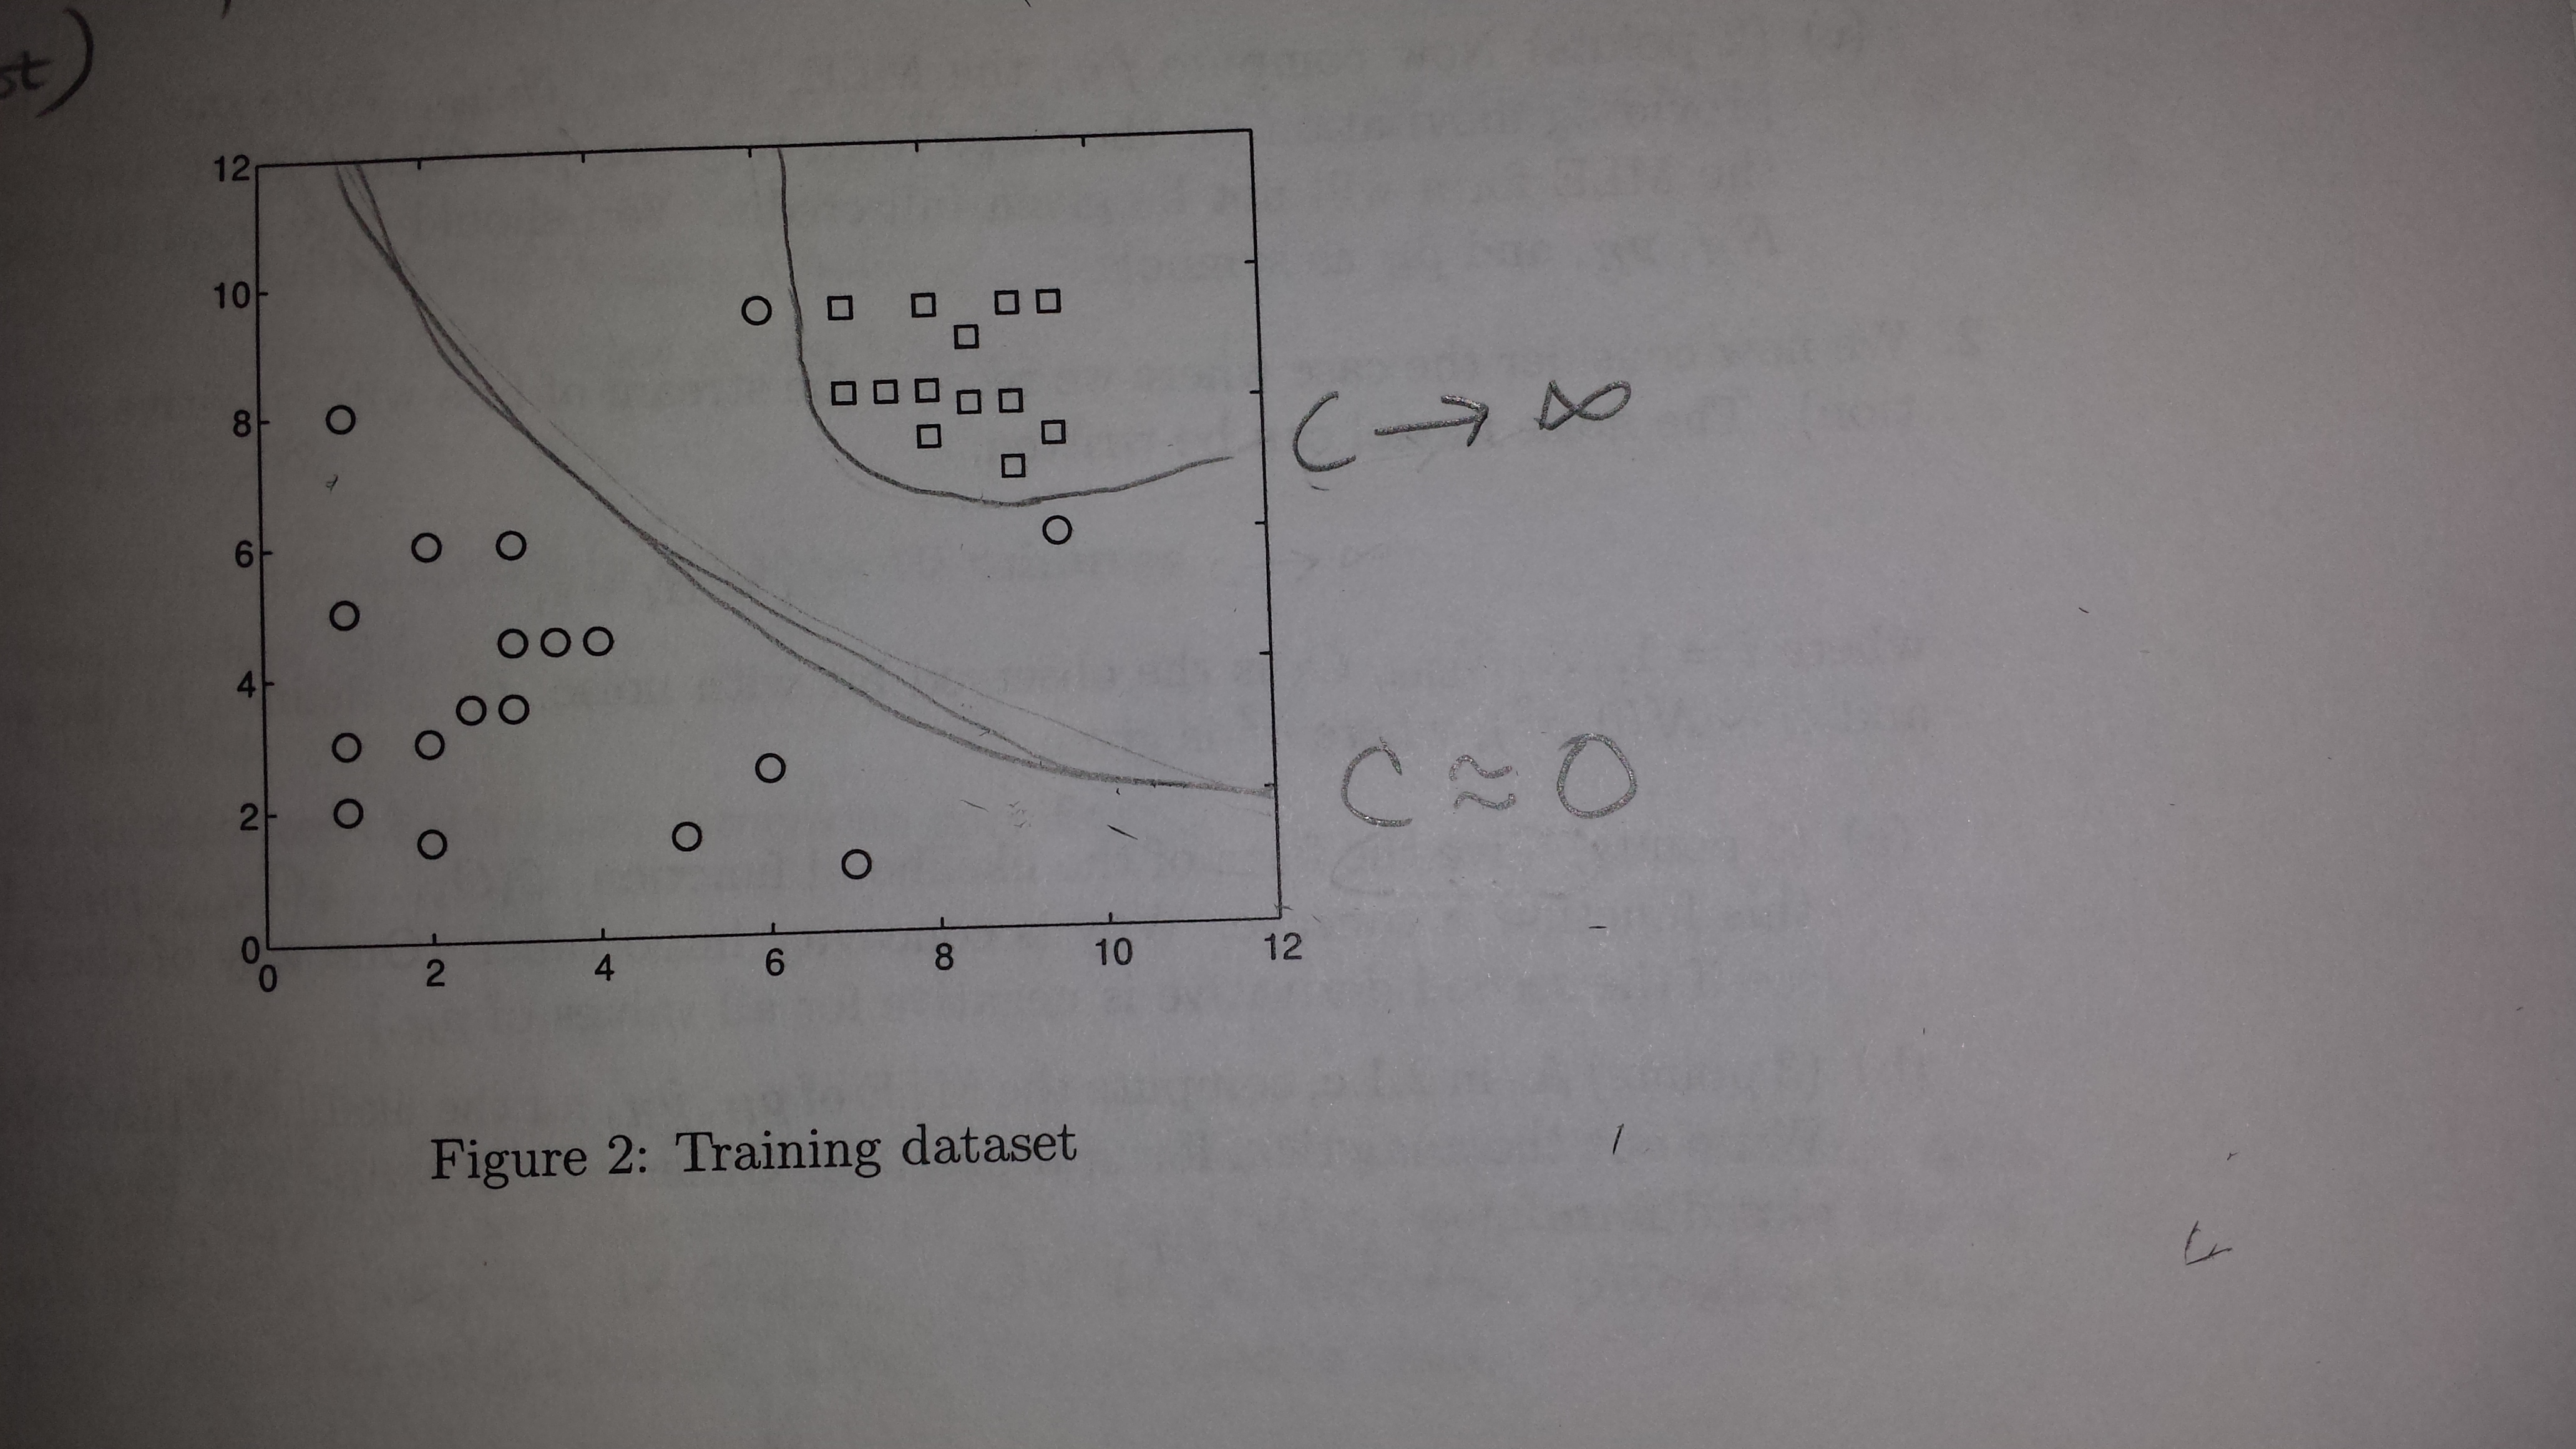
\includegraphics[scale=0.10]{hw2_ques1_2_ab}
		\end{figure}
		\item
		As C approaches infinity, the cost of misclassification is extremely high so the model will try to separate the data exactly.  In this case, it is able to do this since the training data is linearly separable, but the resulting boundary overfits the data. 
		\item
		If C is near 0, then there is no cost to overfitting so 1 or more outlier data points do not determine the decision boundary. This means that we can permit the outliers to be margin errors which results in a decision boundary that is much more general in comparison to the decision boundary produced when the cost approaches infinity.
		\item
		Case (b) would work a lot better in the classification task. Given that the training data is error-prone, using case (a) would be highly inappropriate because it assumes that the training data is noise-free. Case (b) will produce a more general decision boundary that will likely classify the data more successfully than case (a). 
	\end{enumerate}
\end{enumerate}
\end{document}